% arara: xelatex
% arara: xelatex
% arara: xelatex

% options:
% thesis=B bachelor's thesis
% thesis=M master's thesis
% czech thesis in Czech language
% english thesis in English language
% hidelinks remove colour boxes around hyperlinks

\documentclass[thesis=M,english,hidelinks]{FITthesis}[2019/12/23]

% \usepackage{subfig} %subfigures
% \usepackage{amsmath} %advanced maths
% \usepackage{amssymb} %additional math symbols

\usepackage[utf8]{inputenc}

\usepackage{graphicx} % inserting images
\usepackage{dirtree} %directory tree visualisation
\usepackage{listings} % use code listings package
\lstset{
	basicstyle=\ttfamily,
	columns=fullflexible,
	frame=single,
	breaklines=true
}

\usepackage{url}


% list of acronyms
\usepackage[acronym,nonumberlist,toc,numberedsection=autolabel,nomain]{glossaries}
\iflanguage{czech}{\renewcommand*{\acronymname}{Seznam pou{\v z}it{\' y}ch zkratek}}{}
\makeglossaries

\newcommand{\tg}{\mathop{\mathrm{tg}}} %cesky tangens
\newcommand{\cotg}{\mathop{\mathrm{cotg}}} %cesky cotangens

% % % % % % % % % % % % % % % % % % % % % % % % % % % % % % % % % % % 
% % % % % % % % % % % % % % % % % % % % % % % % % % % % % % % % % % % 
\department{Department of theoretical computer science}
\title{Framework for Extraction of Wikipedia Articles Content}
\authorGN{Oleksandr} %author's given name/names
\authorFN{Husiev} %author's surname
\authorWithDegrees{Oleksandr Husiev} %author's name with academic degrees
\author{Oleksandr Husiev} %author's name without academic degrees
\supervisor{Ing. Milan Doj{\v c}inovski, Ph. D.}
\acknowledgements{I would like to thank my supervisor Milan Doj{\v c}inovski, family and friends for their prolonged support during writing this thesis.}
\abstractCS{Tato diplomová práce se zabývá extrakcí obsahu Wikipedie pro DBpedia - crowd-sourced projekt.
	Hlavním cílem této práce bylo vyvinout rámec pro extrakci obsahu, struktury a anotací článků z Wikipedie. Výsledkem  je framework, který zpracovává velké skládky XML na Wikipedii v několika populárních jazycích s možností dynamicky přidávat nové jazyky a vytváří čistý textový výstup, odkazy a strukturu stránky ve formátu N-Triples.}
\abstractEN{This thesis describes the development process of the extraction of Wikipedia articles content for a DBpedia, a crowd-sourced community effort.
The main goal of this thesis was  to develop a framework for extraction of Wikipedia articles content, structure, and annotations.  The result is a framework that processes large Wikipedia XML dumps in several popular languages, with the possibility to dynamically add new languages, and produces clean text output, links, and page structure in N-Triples format.}
\placeForDeclarationOfAuthenticity{Prague} %where you have signed the declaration
\keywordsCS{NIF, RDF, propojená data, web škrábání.}
\keywordsEN{NIF, RDF, linked data, web scraping, knowledge graph.}
\declarationOfAuthenticityOption{4} %select as appropriate, according to the desired license

\begin{document}
	
\newacronym{LOD}{LOD}{Linked Open Data}
\newacronym{RAM}{RAM}{Random Access Memory}
\newacronym{CLI}{CLI}{Command Line Interface}
\newacronym{W3C}{W3C}{World Wide Web Consortium}
\newacronym{FR}{FR}{Functional Requirement}
\newacronym{XML}{XML}{Extensible Markup Language}
\newacronym{NLP}{NLP}{Natural Language Processing}
\newacronym{NIF}{NIF}{\gls{NLP} Interchange Format}
\newacronym{RDF}{RDF}{Resource Description Framework}
\newacronym{OWL}{OWL}{Web Ontology Language}
\newacronym{SKOS}{SKOS}{Simple Knowledge Organization System}
\newacronym{SPARQL}{SPARQL}{SPARQL Protocol and RDF Query Language}
\newacronym{URI}{URI}{Uniform Resource Identifier}
\newacronym{HTTP}{HTTP}{Hypertext Transfer Protocol}
\newacronym{HTML}{HTML}{HyperText Markup Language}
\newacronym{WWW}{WWW}{World Wide Web}
\newacronym{DRY}{DRY}{Don't Repeat Yourself}
\newacronym{FOAF}{FOAF}{Friend Of A Friend}
\newacronym{RSS}{RSS}{\gls{RDF} Site Summary}
\newacronym{CLI}{CLI}{Command Line Interface}
\newacronym{GUI}{GUI}{Graphic User Interface}
\newacronym{REST}{REST}{Representational State Transfer}
\newacronym{API}{API}{Application Programming Interface}
\newacronym{NLP}{NLP}{Natural Language Processing}
\newacronym{NIF}{NIF}{NLP Interchange Format}
\newacronym{JVM}{JVM}{Java Virtual Machine}
\newacronym{IDE}{IDE}{Integrated Development Environment}
\newacronym{POJO}{POJO}{Plain Old Java Object}
\newacronym{J2EE}{J2EE}{Java 2 Platform Enterprise Edition}
\newacronym{JAXB}{JAXB}{Jakarta XML Binding}
\newacronym{CSV}{CSV}{Comma-separated values}
\newacronym{YAML}{YAML}{Yet Another Markup Language}
\newacronym{SHACL}{SHACL}{Shapes Constraint Language}


\begin{introduction}
	
	\section{Motivation}

	Knowledge bases are growing up in importance as a Web and enterprise search engine. At the moment, knowledge bases cover only specific niches and are not useful outside of their primary purpose. As part of a broader DBpedia initiative, this thesis has an objective to structure information, store it in a machine-readable form, and provide better ways for information to be collected, organized, searched, and utilized.

	A DBpedia is a knowledge base, which information is organized as an open knowledge graph. DBpedia data is served as Linked Data, which opens a new way to access the Web for applications: via browser, automated crawlers, or complex SQL-like queries. For example, current technologies do not allow to combine information about cities, criminal rates, climate, and open job postings into one search. The goal of DBpedia is to enable such queries to happen.
	
	The creation of the Framework for Extraction of Wikipedia Articles Content is important as it will allow the DBpedia initiative to receive formatted article data from the Wikipedia on a regular basis. 

	\section{Objectives}

	The main sight of the thesis is to extract structured content from Wikipedia articles. This content can be divided into several main parts: context, structure, and links. Context is the text itself. The structure is how the article is organized and split into sections, subsections and paragraphs, and links are either links to other Wikipedia articles or external websites. Additionally, it is essential to take care of article publication dates, clean up the non-standard articles and sections, and cover other Wikipedia languages.
\begin{enumerate}
	\item Accept and process input data in the form of Wikipedia XML dumps
	\item Extract context.
	\item Extract page structure.
	\item Extract links.
	\item Provide outputs for context, links and page structure in the form of N-Triples.
	\item Implement language extensibility.
	\item Provide a user interface.
\end{enumerate} 

  \section{Challenges}
	The main problem, however, is the current size of Wikipedia. Only a full English Wikipedia dump containing only text and XML structures takes around 16 GB of space. Therefore, a thesis should research the design and implementation of not only functional but an efficient parser with both horizontal and vertical scalability in mind.

	An additional challenge lies in the structure of a general wiki page. Not all pages and their components are structured in the same way. For example, some of the pages might have a line break in the middle of a citation link, that can be ambiguously interpreted as a new paragraph start. This can cause unexpected errors and exceptions during the parsing, and the goal of the project is also to minimize and gracefully handle such exceptions.
	
\end{introduction}

\chapter{Background and related works}

\section{The Concept of Semantic Web}

The Semantic Web is a Web of Data, an extension to the Web that links the related data. The collection of Semantic Web technologies (such as \gls{RDF}, \gls{OWL}, \gls{SKOS}, \gls{SPARQL}, etc.) provides an environment where application can query that data, draw inferences using vocabularies, etc. The goal of the Semantic Web is to develop languages to express current Internet data in a machine processable way. This is achieved by making Internet data interoperable  by allowing every machine to exchange data that has unambiguous meaning defined in centralized reference resources, such as DBPedia."Semantic Web" is a term that Tim Berners-Lee has initially coined\cite{Berners_QA} for a web of data where not simply text, but also meaning, or logical connections that machines can process.
The Semantic Web is an extension of the current World Wide Web, defined by standards set by the \gls{W3C}.

Although Semantic Web is a term that has often been criticized as confusing, opaque, and academic, it does nonetheless capture two of the most critical aspects of these technologies:

\begin{itemize}
	\item  \textbf{Semantic:} The meaning of the data is not only explicitly represented and richly expressive, but it also “travels” along with the data itself;
	\item \textbf{Web:} Individual pieces of data are linked together into a network of information, just as documents are linked together on the World Wide Web.
\end{itemize}

Less familiar synonyms to the Semantic Web are the following: Linked Data Web, the Web of Data, Web 3.0, the Enterprise Information Web, or the Giant Global Graph.

\section{What is Linked Data?}

In order to make Semantic Web, or Web of Data, a reality, it is necessary to support a vast amount of data that are manageable and reachable by a variety of Semantic Web tools. Not only access to data but also relationships among data should be provided. This collection of interconnected datasets can also be referred to as Linked Data.

The term was introduced in 2006 by Tim Berners-Lee's four rules for publishing data on the Web\cite{Berners_LinkedData}, stating the following expectations for \gls{HTML} or \gls{RDF} standards:
\begin{enumerate}
	\item Use \gls{URI} as an identifier.
	\item Use \gls{HTTP} \gls{URI}s so that people can look up those names.
	\item When someone looks up a \gls{URI}, provide useful information, using the standards (\gls{RDF}*, \gls{SPARQL})
	\item Include links to other \gls{URI}s. so that they can discover more things.
\end{enumerate}

While these four rules are the basis of Linked Data and related developments, their exact implementation can be done differently and evolves over time. Specifically, the way \gls{URI} is now serialized either in \gls{RDF}/\gls{XML} or via N3(also known as Turtle, or N-triples).

\subsection{RDF Description}\label{rdf-description}

The Resource Definition Framework(RDF) is a general-purpose language for representing information in the Web\cite{roussey2011}.The \gls{RDF} data model is similar to classical conceptual modeling approaches, such as entity-relationship or class diagrams. It is based on the idea of making statements about the resource in expressions of the form subject–predicate–object, also known as triples. The subject denotes the resource, and the predicate denotes traits or aspects of the resource, and expresses a relationship between the subject and the object\cite{rdf_syntax}.

The underlying structure of any expression in RDF is a collection of triples, each consisting of a subject, a predicate and an object. A set of such triples is called an RDF graph. Each triple represents a statement of a relationship between the things denoted by the nodes that it links. Each triple has three parts - subject, predicate and object\cite{rdf_concepts}. Subject and object are graph nodes, while a predicate defines a relation between them, pointing from subject to an object. On \ref{fig:basicrdfgraph}, for a triple <http://www.w3.org/TR/rdf-syntax-grammar> is a subject, <http://purl.org/de/elements/1.1/title> is a predicate and "RDF/XML Syntax Specification (Revised)" is an object.

\begin{figure}
	\centering
	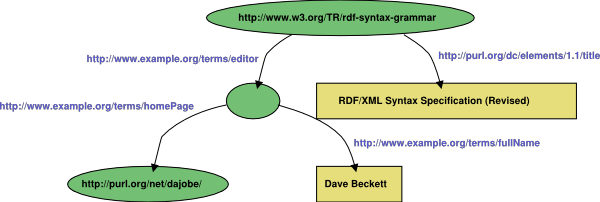
\includegraphics[width=1.0\linewidth]{basic_rdf_graph}
	\caption{Basic RDF Graph\cite{rdf_syntax}}
	\label{fig:basicrdfgraph}
\end{figure}

To define what a subject is, we need to define an \gls{RDF} \gls{URI} Reference.

\textbf{\gls{RDF} \gls{URI} Reference} - is a Unicode string that:

\begin{itemize}
	\item does not contain any control characters ( \#x00 - \#x1F, \#x7F-\#x9F)
	\item and would produce a valid URI character sequence (per RFC2396\cite{rfc2396}, sections 2.1) representing an absolute URI with optional fragment identifier when subjected to the encoding described below.
\end{itemize}

\textbf{Blank node} is a special case for \gls{RDF} graph nodes that do not have a \gls{URI} Reference, usually represented as "\_". Those blank nodes represent all nodes for which graph only has partial information in a form of this node's objects.

\textbf{Literal} is a node that is used to identify values such as numbers, strings or dates by means of a lexical representation. Literal can be either plain or typed. For plain literals, they represented by a text and an optional language tag. For typed literals, they are represented by a string and a type tag, for example in <xsd:boolean, "false"> xsd:boolean is a type and  "false" is a string of a type boolean.

Subject can be either an \gls{RDF} \gls{URI} Reference or a blank node. 
Predicate is an \gls{RDF} \gls{URI} Reference.
Object can be an \gls{RDF} \gls{URI} Reference, Literal or a blank node.

In applications of RDF such as \gls{RSS} resources are represented by URIs that denote and are used to link actual data on the World Wide Web\cite{rdf_concepts}. \gls{RDF} in general can be used not only for Internet resources, but for other knowledge ontologies too.

An \gls{RDF} database, also called triplestore contains triples of  interrelated statements that can be visualized with a network graph. A traditional relational database might split attributes about artworks and features about artists into separate tables. In an RDF/graph database, all these data points belong to the same interconnected graph, allowing users maximum flexibility in deciding how they wish to query it.

RDF graphs can also be represented in many text serialization formats. In a sentence "Mona Lisa was painted by Leonardo da Vinci" the subject is  "Mona Lisa", the object is "Leonardo da Vinci" , and a predicate  that defines a relation between the subject and the object is "paintedBy", as  seen in the listing \ref{lst:rdf-statement} .

\begin{lstlisting}[language=XML, caption=Example of an RDF statement, label = {lst:rdf-statement}]
<https://dbpedia.org/page/Mona_Lisa> <http://purl.org/dc/terms/title> "Mona Lisa" .

<https://dbpedia.org/ontology/author> <http://www.w3.org/1999/02/22-rdf-syntax-ns#label> "was created by" .

<https://dbpedia.org/page/Leonardo_da_Vinci> <http://xmlns.com/foaf/0.1/name> "Leonardo da Vinci" .
\end{lstlisting}

The particular encoding for resources or triples varies from format to format. A non-exhaustive list of popular \gls{RDF} serialization formats includes:
\begin{itemize}
	\item \textbf{Turtle} - a compact human-friendly format.
	\item \textbf{N3} - format that is similar to Turtle, but allows for additional features like inference, or transformation rules.
	\item \textbf{N-Triples} - a very simple, easy-to-parse, line-based format that is not as compact as Turtle.
	\item \textbf{N-Quads} - a superset of N-Triples for serializing multiple \gls{RDF} graphs.
	\item \textbf{RDF/XML} - an XML-based syntax that was the first standard format for serializing RDF.
	\item \textbf{RDF/JSON} - an alternative syntax for expressing RDF triples using a simple JSON notation.
	\item \textbf{JSON-LD} - a JSON-based serialization, allows data to be serialized in a way that is similar to traditional JSON. 
\end{itemize}

For example, it is required to write an \gls{RDF} file,  say \textless http://example.org/smith\textgreater, local identifiers, say  \#albert, \#brian and \#carol.  This  \gls{RDF} file will look differently in \gls{XML}(\ref{lst:rdf-xml-example}), Turtle format(\ref{lst:rdf-turtle-example}). It can be observed that Turtle format is more concise than the \gls{XML} one.

\begin{lstlisting}[language=XML, caption=Example of RDF serialization in XML, label = {lst:rdf-xml-example}]
<rdf:Description about="#albert"
	<fam:child rdf:Resource="#brian">
	<fam:child rdf:Resource="#carol">
</rdf:Description>
\end{lstlisting}


\begin{lstlisting}[language=XML, caption=Example of RDF serialization in N3/Turtle, label = {lst:rdf-turtle-example}]
	<#albert>  fam:child <#brian>, <#carol>.
\end{lstlisting}

The \gls{WWW} architecture now gives a global identifier  "http://example.org/smith\#albert" to Albert. Anyone can now use this global identifier to refer to and provide more information about Albert.

In addition to describing a link, it is essential to know when to make a link. One important pattern is a set of data which you can explore as you go link by link by fetching data.   Whenever one looks up the \gls{URI} for a node in the RDF graph, the server returns information about the arcs out of that node, and the arcs in.  In other words, it returns any RDF statements in which the term appears as either subject or object.

Formally, call a graph G \textit{browsable} if, for  the \gls{URI} of any node in G, if I look up that \gls{URI} I will be returned information which describes the node, where describing a node means:
\begin{enumerate}
	\item Returning all statements where the node is a subject or object; and
	\item Describing all blank nodes attached to the node by one arc.
\end{enumerate}

There are also the next limitations on such browseable data, mainly regarding data consistency across separate documents. By these definitions, statements which relate things in two different documents must be repeated. This clearly goes against the knowledge principle \gls{DRY}, or in this case, not to store data in other places, as the problems with keeping the data consistent will arise eventually. A set of completely browsable data with links in both directions has to be completely consistent, and that takes coordination, especially if different authors or programs are involved.

One of the solutions to this repetition problem is to have links of a certain property in a separate document.   A person's homepage doesn't list all their publications but instead puts a link to it a separate document listing them.

In conclusion, linked data is essential for linking the Semantic Web. It is quite easy to implement linked data in both new and already existing applications or websites. Various common-sense considerations determine when to make a link and when not to.

\section{NLP Interchange Format}

\gls{NLP} is a field of science that combines lingustics, computer science and artificial intelligence concerned with the interactions between computers and human language, in particular how to program computers to process and analyze large amounts of natural language data.

The \gls{NIF} is an \gls{RDF}/\gls{OWL}-based format that aims to achieve between \gls{NLP} tools, language resources and annotations\cite{nlp_cite}. NIF consists of specifications, ontologies and software  that are combined under the  version identifier "NIF 2.0", but are also versioned separately. The initial specification of \gls{NIF} was released in November 2011.

\gls{NIF} is being developed as a result and to facilitate the needs of Linked Data and related tools.  NIF addresses the interoperability problem on three layers: the structural, conceptual and access layer. NIF is based on a Linked Data enabled URI scheme for identifying elements in (hyper-)texts that are described by the NIF Core Ontology (structural layer) and a selection of ontologies for describing common NLP terms and concepts (conceptual layer). NIF-aware applications will produce output adhering to the NIF Core Ontology as REST services (access layer). NIF enables the creation of heterogeneous, distributed and loosely coupled NLP applications, which use the Web as an integration platform. Another benefit is
that a NIF wrapper has to be only created once for a particular tool, but enables the tool to interoperate with a potentially large number of other tools without additional adaptations. Ultimately, we envision an ecosystem of NLP tools and services to emerge using NIF for exchanging and integrating rich annotations.

\gls{NIF} consists of several core components that are described below.

\paragraph{URI Schemes}

The idea behind NIF is to allow NLP tools to exchange annotations about text in RDF. Hence, the main prerequisite is that text becomes referenceable by URIs, so that they can be used as resources in RDF statements\cite{linked_data_uri}\cite{workflow_modularity}. In NIF, there is a distinction between the document $d$, the text $t$ contained in the document and possible substrings $s_{t}$ of this text.  We call an algorithm to systematically create identifiers for $t$ and $s_{t}$ a \textit{URI Scheme}.  The canonical URI scheme of NIF is based on RFC 5147\cite{nif_rdf}, which standardizes fragment ids for the text/plain media type. According to RFC 5147, the following URI can address the first occurrence of the substring “Semantic Web” in the
text (26610 characters) of the document \url{http://www.w3.org/DesignIssues/LinkedData.html} with the separator \#: \url{http://www.w3.org/DesignIssues/LinkedData.html\#char=717,729}.

\paragraph{NIF Core Ontology}



The NIF Core Ontology\cite{nif_core_ontology} provides classes and properties to describe the relations between substrings, text, documents and their URI schemes. The main class in the ontology is nif:String, which is the class of all words over the alphabet of Unicode characters (sometimes called $\Sigma^{*}$). We built NIF upon the Unicode Normalization Form C, as this follows the recommendation of the RDF standard for rdf:Literal. Indices are to be counted in code units. Each URI scheme is a subclass of nif:String and puts further restrictions over the syntax of the URIs. For example, instances of type nif:RFC5147String have to adhere to the NIF URI scheme based on RFC 5147. Users of NIF can create their own URI schemes by subclassing nif:String and providing documentation on the Web in the rdfs:comment field.

Framework for Extraction of Wikipedia Articles Content generates a resource of the nif:Context OWL class. This class is assigned to the whole string of the text (i.e. all characters). The purpose of an individual of this class is special, because the string of this individual is used to calculate the indices for all substrings. Therefore, all substrings have to have a relation nif:referenceContext pointing to an instance of nif:Context.

\subsection{Existing Use Cases for NIF}

\paragraph{Internationalization Tag Set}
The \textit{Internationalization Tag Set (ITS)} Version 2.0 is a W3C working draft, which is in the final phase of becoming a W3C recommendation. Among other things, ITS standardizes HTML and XML attributes which can be leveraged by the localization industry (especially language service providers) to annotate HTML and XML nodes with processing information for their data value chain.

An example of three attributes in an HTML document is given here\ref{lst:its-example}:

\begin{lstlisting}[language=HTML, caption=Example of Internationalization Tag Set HTML Code, label = {lst:its-example}]
<html> 
	<body>
	<h2 translate="yes"> 
		Welcome to <span its-ta-ident-ref="http://dbpedia.org/resource/Dublin" its-within- text="yes" translate ="no"> Dublin </span> in <b translate ="no" its-within-text="yes"> Ireland </b>! 
	</h2> 
	</body> 
</html>
\end{lstlisting}

NIF successfully creates a bridge between ITS and RDF and a round-trip conversion was recently implemented as a proof-of-concept. Therefore, NIF can be expected to receive a wide adoption by machine translation and industrial language service providers. Additionally, the ITS Ontology provides well modeled and accepted properties, which can in turn be used to provide best practices for NLP annotations.

\paragraph{Ontologies of Linguistic Annotation}

The Ontologies of Linguistic Annotation (OLiA) provide stable identifiers for morpho-syntactical annotation tag sets, so that NLP applications can use these identifiers as an interface for interoperability. OLiA provides Annotation Models (AMs) for fine-grained identifiers of NLP tag sets. The
individuals of these annotation models are then linked via rdf:type to coarse-grained classes from a Reference Model (RM), which provides the interface for applications. NIF provides two properties: nif:oliaLink links a nif:String to an OLiA Annotation Model. Although a reasoner could automatically deduce the abstract type of each OLiA individual from the RM, it was a requirement that the coarse-grained types should be linked redundantly to the strings as well in case reasoning services are not available or would cause high overhead. Therefore, an OWL annotation property nif:oliaCategory was created as illustrated in the following example\cite{lst:olia-example}.

\begin{lstlisting}[language=HTML, caption=Example of Internationalization Tag Set HTML Code, label = {lst:olia-example}]
<char=342,345> a nif:String, nif:RFC5147String;
nif:oliaLink penn:NNP;
nif:oliaCategory olia:Noun, olia:ProperNoun .
# deducable by a reasoner :
penn:NNP a olia:Noun, olia:ProperNoun .
\end{lstlisting}


\section{Linked Open Data and DBpedia}

A typical example of a large Linked Dataset is DBpedia. DBpedia and related tools are supported by the Leipzig University research group. As stated in the related article, is a community effort to extract structured information from Wikipedia and to make this information available on the Web. DBpedia allows internet users to ask sophisticated queries against datasets derived from Wikipedia and to link other datasets on the Web to Wikipedia data. This section will describe the extraction of the DBpedia datasets, and how the resulting information is published on the Web for human and machine consumption\cite{dbpedia_nucleus}.

The most effective way of spurring synergistic research along these directions is to provide a rich corpus of diverse data. This would enable researchers to develop, compare, and evaluate different extraction, reasoning, and uncertainty management techniques, and to deploy operational systems on the Web. The DBpedia project has derived such a data corpus from the Wikipedia encyclopedia.

Wikipedia editions are available in over 250 languages, with the English one accounting for more than 1.95 million articles. Like many other web applications, Wikipedia has the problem that its search capabilities are limited to full-text search, which only allows very limited access to this valuable knowledge base. As has been highly publicized, Wikipedia also exhibits many of the challenging properties of collaboratively edited data: it has contradictory data, inconsistent taxonomical conventions, errors, and even spam. 

The DBpedia project focuses on the task of converting Wikipedia content into structured knowledge, such that Semantic Web techniques can be employed against it — asking sophisticated queries against Wikipedia, linking it to other datasets on the Web, or creating new applications or mashups.

The DBpedia project focuses on the task of converting Wikipedia content into structured knowledge, such that Semantic Web techniques can be employed against it — asking sophisticated queries against Wikipedia, linking it to other datasets on the Web, or creating new applications or mashups. DBpedia project makes the following contributions:
\begin{itemize}
	\item Develop an information extraction framework, which converts Wikipedia
	content to RDF. The basic components form a foundation upon which further research into information extraction, clustering, uncertainty management, and query processing may be conducted.
	\item Provide Wikipedia content as a large, multi-domain RDF dataset, which
	can be used in a variety of Semantic Web applications. The DBpedia dataset
	consists of 103 million RDF triples.
	\item Iinterlink the DBpedia dataset with other open datasets. This results in
	a large Web of data containing altogether around 2 billion RDF triples.
	\item Develop a series of interfaces and access modules, such that the dataset
	can be accessed via Web services and linked to other sites.
\end{itemize}

\subsection{Extracting Structured Information from Wikipedia}
Wikipedia articles contain different types of structured information, such as infobox templates, categorisation information, images, geo-coordinates, links to external Web pages and links across different language editions of Wikipedia. To process this, Wikipedia uses Mediawik software. Due to the nature of this  Wiki system, basically all editing, linking, annotating with meta-data is done inside article texts by adding special syntactic constructs. Hence, structured information can be obtained by parsing article texts for these syntactic constructs. Example of Wikipedia XML and then cleaned text that will be shown to the user can be seen in listings \ref{lst:raw-wikipedia-xml} and \ref{lst:cleaned-wikipedia-text} respectively. 

\begin{lstlisting}[caption=Raw Wikipedia XML,frame=tlrb,  label = {lst:raw-wikipedia-xml}]{Name}
{{basic forms of government}}
'''Anarchism''' is an [[Anti-authoritarianism|anti-authoritarian]] [[Political philosophy|political]] and [[Social philosophy|social philosophy]]{{sfnm|1a1=McLaughlin|1y=2007|1p=59|2a1=Flint|2y=2009|2p=27}} that rejects [[Hierarchy|hierarchies]] deemed unjust and advocates their replacement with [[Workers' self-management|self-managed]], [[Self-governance|self-governed]] societies based on voluntary, [[cooperative]] institutions. These institutions are often described as [[Stateless society|stateless societies]],{{sfnm|1a1=Sheehan|1y=2003|1p=85|2a1=Craig|2y=2005|2p=14}} ...
\end{lstlisting}

\begin{lstlisting}[caption=Cleaned Wikipedia text,frame=tlrb, label = {lst:cleaned-wikipedia-text}]{Name}
Anarchism is an anti-authoritarian political and social philosophy that rejects hierarchies deemed unjust and advocates their replacement with self-managed, self-governed societies based on voluntary, cooperative institutions. These institutions are often described as stateless societies, ...
\end{lstlisting}

The XML extraction algorithm detects such Mediawiki templates and recognizes their structure using pattern matching techniques. It selects significant templates, which are then parsed and transformed to RDF triples. The algorithm uses post-processing techniques to increase the quality of the extraction. MediaWiki links are recognized and transformed to suitable URIs, common units are detected and transformed to data types. Furthermore, the algorithm can detect lists of objects, which are transformed to RDF lists.

\subsection{DBpedia Dataset}

As stated on the DBpedia's official website\cite{DBpedia_facts}, the English version of the DBpedia dataset currently provides information about more than 4.58 million things, out of which 4.22 million are classified in a consistent ontology, including at least 1,445,000 persons, 735,000 places(including 478.000 populated places), 411,000 creative works (including 123,000 music albums, 87,000 films and 19,000 video games), 241,000 organizations (including 58,000 companies and 49,000 educational institutions), 251,000 species and 6,000 diseases.

DBpedia concepts are described by short and long abstracts in 125 languages. All these versions together describe 38.3 million things, out of which 23.8 million are localized descriptions of things that also exist in the English version of DBpedia. The full DBpedia data set features 38 million labels and abstracts in 125 different languages, 25.2 million links to images and 29.8 million links to external web pages; 80.9 million links to Wikipedia categories, and 41.2 million links to YAGO categories. DBpedia is connected with other Linked Datasets by around 50 million RDF links.

\subsection{Triplestore}

A triplestore is a software program capable of storing and indexing RDF data, in order to enable querying this data efficiently. Most triplestores support the SPARQL query language for querying RDF data. Virtuoso, Sesame, and BigOWLIM are typical examples of triplestores. DBpedia is using Virtuoso as the underlying triplestore.

\subsection{DBpedia Dataset Web Endpoints}

DBpedia website provides three access mechanisms to the DBpedia dataset: Linked Data, the SPARQL protocol, and downloadable RDF dumps. Royalty-free access to these interfaces is granted under the terms of the GNU Free Documentation License\cite{dbpedia_live_sparql}.

\textit{Linked Data.} DBpedia resource identifiers, are set up to return RDF descriptions when accessed by Semantic Web agents, and a simple HTML view of the same information to traditional web browsers. HTTP content negotiation is used to deliver the appropriate format.

\textit{SPARQL Endpoint.} Client applications can send queries over the SPARQL protocol to this
endpoint at http://dbpedia.org/sparql. This interface is appropriate when the client application developer knows in advance exactly what information is needed. In addition to standard SPARQL, the endpoint supports several extensions of the query language that have proved useful for developing user interfaces: full text search over selected RDF predicates, and aggregate functions, notably COUNT. To protect the service from overload, limits on query cost and result size are in place. For example, a query that asks for the store’s entire contents is rejected as too costly, and SELECT results are truncated at 1000 rows.

\textit{RDF Dumps.} N-Triple serializations of the datasets are available for download at the DBpedia website and can be used by sites that are interested in larger parts of the dataset.

\section{Related works}

\subsection{DBpedia Information Extraction Framework}\label{dbpedia_in_extraction_framework}
Prior to the current project, a few projects have already been made in order to facilitate DBpedia's need for extracting information from Wikipedia and related resources, namely \textbf{DBpedia Information Extraction Framework}\cite{dbpedia_live_extraction}. 

DBpedia Information Extraction Framework focuses on the main disadvantage of DBpedia: heavy-weight release process. Producing a DBpedia dataset release through the traditional dump-based extraction requires manual effort and – since dumps of the Wikipedia database are created on a monthly basis – DBpedia has never reflected the current state of Wikipedia. Hence, this project extended the DBpedia extraction framework to support a \textit{live extraction}, which works on a continuous stream of updates from Wikipedia and processes that stream on the fly. More importantly, the extraction framework focuses on other parts of the Wikipeida articles. The framework has 19 extractors that process the following Wikipedia content, most important of which are list below:
\begin{itemize}
	\item \textit{Labels.} All Wikipedia articles have a title, which is used as an rdfs:label for the
	corresponding DBpedia resource.
	\item \textit{Abstracts.} Those include a short abstract (first paragraph, represented by using rdfs:comment) and a long abstract (text before a table of contents, using the 	property dbpedia:abstract) from each article.
	\item \textit{Interlanguage links. }
	\item \textit{Images.}
	\item \textit{Redirects.}
	\item \textit{Disambiguation.}
	\item \textit{External links.}
	\item \textit{Page links.}
	\item \textit{Person data.} It extracts personal information such as surname, and birth date.	This information is represented in predicates such as foaf:surname, and dbpedia:birthDate.
	\item \textit{Infobox}
	\item \textit{Category label} Wikipedia articles are arranged in categories, and this extractor	extracts the labels for those categories.
\end{itemize}


\chapter{Analysis and Implementation}

\section{Requirements}\label{framework_requirements}

Before starting to design the project, it is beneficial to specify the requirements. There several ways to layout the requirements, mainly writing down formal requirements or use cases. Because the project is oriented on delivering results to a smaller group of developers, it will be better to use formal requirements, as opposed to user-oriented use cases.

The list of functional requirements for the Framework for Extraction of Wikipedia Articles Content:

\begin{enumerate}
	\item \textbf{Accept input data:} The framework should accept the official  Wikipedia dumps in the \gls{XML} format, provided by the Wikipedia. The dumps can contain an amount of information up to 20 GB of text data. The framework should be able to parse dumps in English and at least 4 other popular Wikipedia languages.
	\item \textbf{Provide outputs:} The framework should print all the outputs in the N-Triples format, concatenating processed data from all articles in a single \gls{XML} input file and writing the data to .nt output file.
	\item \textbf{Extract context:} The framework should extract clean text from the Wikipedia page, removing or processing all the \gls{XML} and Wikipedia-specific markup, including the core text but excluding infoboxes, files, images, and footers.
	\item \textbf{Extract page structure:} The framework should extract a page tree, where every page section is a node, preserving the relation to the page context. The page tree should include The page tree should be printed in an output file separately from the page context. 
	\item \textbf{Extract links:} In addition to context, the framework should supplement the context by extracting internal Wikipedia links from the page. These links should refer to their respective sections of the text, and include only other Wikipedia articles, excluding possible external links to other web pages. The links should also be printed in another output file, separately from the page structure and context.
	\item \textbf{Implement extensibility:} The framework should be easily extensible by other developers to include new languages.
	\item \textbf{Provide an interface:} The framework is required to have an intuitive interface for the user to easily leverage the framework in other works.
	\item \textbf{Evaluate the results:} The framework should contain the metrics that will provide user with a feedback about every execution.
\end{enumerate} 

While functional requirements are the most important part of the project, there can be other, less specific requirements that go along with the functional requirements, commonly known as non-functional requirements. For this project, the non-functional requirements were next:

\begin{enumerate}
	\item  Research of Wikipedia \gls{XML} Dump Structure and \gls{NIF} data format.
	\item  Find ways to facilitate the goals of the DBpedia project.
\end{enumerate}

\subsection{Desired Output}

The output that is required is defined below\cite{NIF_Format}, split into context, links and page structure. 


\subsubsection{Context}

Context is a resource that includes the full text of a page with all the Wikipedia formatting removed in a nif:isString property. This string serves as a context for its substrings. The Unicode String given in the nif:isString property must be used to calculate the begin and endIndex for all nif:Strings that have a nif:referenceContext property to this URI\cite{NIF_Ontology}.For the context resource, we need next values:

\begin{itemize}
	\item \textbf{Predicate Language - predLang.} The main language of the context. 
	\item \textbf{Context String - isString.} The context's text.
	\item \textbf{Source URL - sourceUrl} Link to the Wikipedia article.
	\item \textbf{Context's Index at the start - beginIndex} Starting index of the context - always starts at zero.
	\item \textbf{Context's Index at the end - endIndex} The context's length.
\end{itemize}

\begin{lstlisting}[caption=Example of an output for context in NIF format,frame=tlrb,  label = {lst:nif-context}]{Name}
@prefix ns0: <http://persistence.uni-leipzig.org/nlp2rdf/ontologies/nif-core#> .
@prefix xsd: <http://www.w3.org/2001/XMLSchema#> .

<http://dbpedia.org/resource/Anarchism?dbpv=2022-02&nif=context>
	ns0:predLang <http://lexvo.org/id/iso639-3/eng> ;
	ns0:sourceUrl <http://en.wikipedia.org/wiki/Anarchism> .

<http://dbpedia.org/resource/Anarchism?dbpv=2022-01&nif=context>
	ns0:isString "Anarchism is an anti-authoritarian political and social philosophy that rejects ..." ;
	ns0:endIndex "43346"^^xsd:nonNegativeInteger ;
	ns0:beginIndex "0"^^xsd:nonNegativeInteger ;
	a ns0:Context .
\end{lstlisting}

\subsubsection{Links}

For the links resource, we need to pick all the internal, or Wikipedia links, as well as external links that lead to other websites from Wikipedia. Note that this does not include references, only links that are part of the text. Links can be either of type Word, which is a single word, or Phrase, which is includes several words that have the same link. Links should have next properties:

\begin{itemize}
	\item \textbf{Reference Context - referenceContext.} The context resource to where this link belongs.
	\item \textbf{Identity Reference - taIdentRef.} Resource's identity reference in DPpedia
	\item \textbf{Super string - superString.} Parent paragraph of the link.
	\item \textbf{Anchor - anchorOf} Link's word or phrase in the text.
	\item \textbf{Context's Index at the start - beginIndex} Starting index of the link, as related to the context's text.
	\item \textbf{Context's Index at the end - endIndex} The link's end index.
\end{itemize}


\begin{lstlisting}[caption=Example of an output for a Word link in NIF format,frame=tlrb,  label = {lst:nif-links}]{Name}
@prefix ns0: <http://persistence.uni-leipzig.org/nlp2rdf/ontologies/nif-core#> .
@prefix xsd: <http://www.w3.org/2001/XMLSchema#> .
@prefix ns1: <http://www.w3.org/2005/11/its/rdf#> .

<http://dbpedia.org/resource/Anarchism?dbpv=2022-02&nif=word_157_170>
	a <http://persistence.uni-leipzig.org/nlp2rdf/ontologies/nif-core#Word> ;
	ns0:referenceContext <http://dbpedia.org/resource/Anarchism?dbpv=2022-02&nif=context> ;
	ns0:beginIndex "157"^^xsd:nonNegativeInteger ;
	ns0:endIndex "170"^^xsd:nonNegativeInteger ;
	ns0:superString <http://dbpedia.org/resource/Anarchism?dbpv=2022-02&nif=paragraph_0_550> ;
	ns1:taIdentRef <http://dbpedia.org/resource/Self-governance> ;
	ns0:anchorOf "self-governed" .
\end{lstlisting}

\subsubsection{Page Structure}

Page structure describes the structure of the article, with sections and paragraphs organize into a tree. Page structure has two types of resources, sections that are separated by titles in the article, and paragraphs that are part of the section.

\begin{itemize}
	\item \textbf{Reference Context - referenceContext.} The context resource to where the page structure belongs.
	\item \textbf{Has Section - hasSection.} Section's children subsections.
	\item \textbf{Has Paragraph - hasParagraph.} Section's paragraphs.
	\item \textbf{First Paragraph - firstParagraph} First paragraph of the section
	\item \textbf{Last Paragraph - lastParagraph} Last Paragraph of the section.
	\item \textbf{Context's Index at the start - beginIndex} Starting index of the section, as related to the context's text.
	\item \textbf{Context's Index at the end - endIndex} The section's end index.
\end{itemize}

\begin{lstlisting}[caption=Example of an output for a Section,frame=tlrb,  label = {lst:nif-links}]{Name}

@prefix ns0: <http://persistence.uni-leipzig.org/nlp2rdf/ontologies/nif-core#> .
@prefix xsd: <http://www.w3.org/2001/XMLSchema#> .

<http://dbpedia.org/resource/Anarchism?dbpv=2022-02&nif=section_0_1231>
	a <http://persistence.uni-leipzig.org/nlp2rdf/ontologies/nif-core#Section> ;
	ns0:hasSection <http://dbpedia.org/resource/Anarchism?dbpv=2022-02&nif=section_3745_3758>, <http://dbpedia.org/resource/Anarchism?dbpv=2022-02&nif=section_1231_3745>, <http://dbpedia.org/resource/Anarchism?dbpv=2022-02&nif=section_43313_43346> ;
	ns0:hasParagraph <http://dbpedia.org/resource/Anarchism?dbpv=2022-02&nif=paragraph_550_1227>, <http://dbpedia.org/resource/Anarchism?dbpv=2022-02&nif=paragraph_0_550> ;
	ns0:referenceContext <http://dbpedia.org/resource/Anarchism?dbpv=2022-02&nif=context> ;
	ns0:lastParagraph <http://dbpedia.org/resource/Anarchism?dbpv=2022-02&nif=paragraph_550_1227> ;
	ns0:endIndex "1231"^^xsd:nonNegativeInteger ;
	ns0:firstParagraph <http://dbpedia.org/resource/Anarchism?dbpv=2022-02&nif=paragraph_0_550> ;
	ns0:beginIndex "0"^^xsd:nonNegativeInteger .
\end{lstlisting}



\section{Design}

\section{General Workflow}

The general data workflow of the Framework for Extraction of Wikipedia Articles is depicted in Figure \ref{fig:general-architecture}.

\begin{figure}
	\centering
	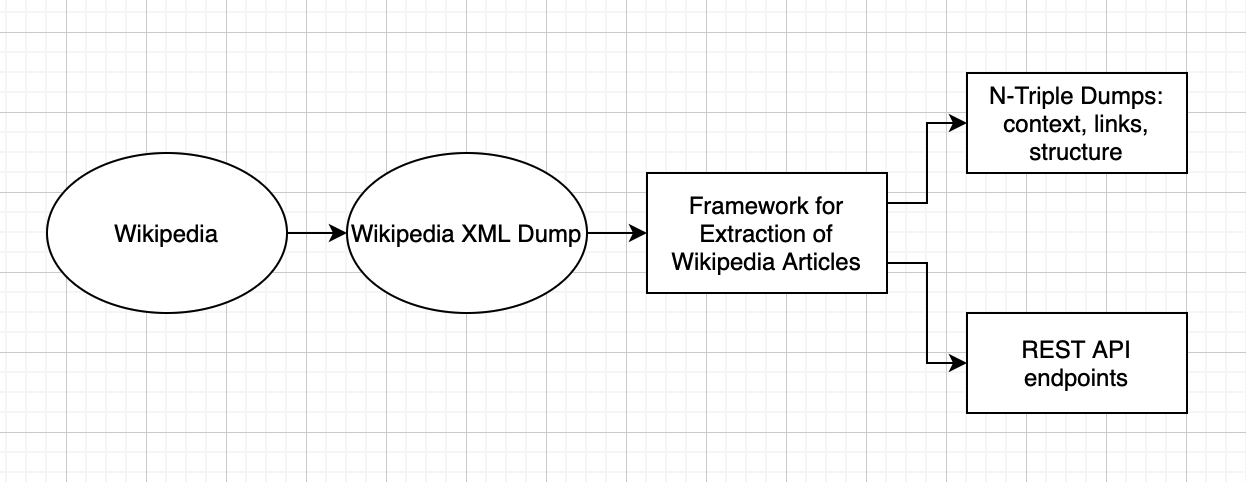
\includegraphics[width=1.0\linewidth]{general_architecture}
	\caption{General Extraction Framework data workflow}
	\label{fig:general-architecture}
\end{figure}

\begin{itemize}
	\item Wikipedia: the main Wikipedia website is the primary sources of information.
	\item Wikipedia XML dump: Wikipedia runs a daily database archivation process and releases all the archived data in the form of XML dumps. These dumps can then be downloaded, unpacked and fed to the framework.
	\item Framework for Extraction of Wikipedia Articles:  the framework processes the XML dump to get the context, structure and links and provide several options for the output.
	\item N-Triples Dumps: one of the outputs is to write the processed information to text files as N-Triples
	\item REST API endpoints: the other option is to provide the REST API endpoints for more convenient view of the output.
\end{itemize}


\section{Usability considerations}\label{usability_considerations}

One of the goals of the application is to make it easy to use, both by researchers and machines. In order to achieve that, application provides several interfaces. For the machines, it might be easier to connect to the application via \gls{REST} \gls{API}. Humans prefer other interfaces, such as \gls{GUI}, or \gls{CLI}.

\subsection{REST API}

\gls{REST} is a software architecture that defines a set of constraints to be used for creating Web services. The Representational State Transfer (REST) style is an abstraction of the architectural elements within a distributed hypermedia system. REST ignores the details of component implementation and protocol syntax in order to focus on the roles of components, the constraints upon their interaction with other components, and their interpretation of significant data elements. It encompasses the fundamental constraints upon components, connectors, and data that define the basis of the Web architecture, and thus the essence of its behavior as a network-based application\cite{rest_proposal}. Web services that implement the REST architecture provide a way to communicate between different internet actors.

An \gls{API} is a client-server interface which defines a contract between clients and servers.

In a RESTful Web service, requests made to a server's API Endpoint will elicit a response with a payload formatted in HTML, XML, JSON, or some other format.

The framework gives an option to use REST API endpoints over the CLI interface. While REST API is a tool used for client-server communication, DBPedia and this Framework also focus on application-based development, where no server communication is needed and all the data and tools are already downloaded and on the client side. This allows for an offline processing, as compared to constant online communication that is required if the parsing tool is only available as a server. WIth this in mind, we can conclude that while \gls{REST} \gls{API} is useful for some particular tasks, it is better to use it as a secondary interface for the Framework.

\subsubsection{REST API Endpoints}

In \gls{API} terminology, communication endpoint, or simply endpoint is a unique URL address that users can access to exchange information with the server. Or in other words, APIs work using requests and responses. When an API requests information from a web application or web server, it will receive a response. The place that APIs send requests and where the resource lives, is called an endpoint\cite{REST_Design}. 

The framework provides the next \gls{REST} endpoints:

\begin{itemize}
	\item \textbf{POST /articles} - Submission endpoint allows you to submit the XML dump or its part to the server. After that is done, the server will asynchronously parse the provided XML, adding the articles to the database as it goes through the submitted articles.
	\item \textbf{GET /articles/\{title\}/context} Get the context N-Triples of an article with a given title.
	\item \textbf{GET /articles/\{title\}/structure} Similarly, get the page structure of an article.
	\item \textbf{GET /articles/\{title\}/links} Get the links associated with an article with a given title.
	\item \textbf{GET /articles/count} Get the total count of articles in a server's database.
\end{itemize}

\subsection{Command Line Interface}

Parsing of large xml files imposes limitations on the technologies that can be used. Particularly, the size of English part of the Wikipedia xml dump has a size of 16 GB. This means that the file cannot be normally loaded into \gls{RAM}, as a single modern computer will usually have from 4 to 16 GB of \gls{RAM}, with Java heap utilizing a quarter of that capability by default. 

Furthermore, modern internet communication is better built around frequent exchange with small packets, and imposes a limit of maximum amount of requests that can be sent in a second. For example, it will not be possible to use Wikipedia's API for this task, as the Wikipedia's server might ban all further requests. For that reason, all the processing should be done offline and not rely on the internet connection at all.

Considering the limitations described above, it was decided to use \gls{CLI} as the main way to use the application. 

To simplify further development process, it was decided to use an existing picocli library for simple CLI implementation, as it reduces the development time by encapsulating most of the CLI-related code, allowing the developer to control only the commands needed for CLI.

\subsection{Command Line Input Options}

The library used to create a \gls{CLI} provides a good mechanisms to generate help text, from which the list of possible arguments, both mandatory and optional, can be extracted:

\begin{itemize}
	\item  \textbf{\textless xmlFile\textgreater} - The relative path to the XML Wiki dump.
	\item \textbf{-c, --clean} - The optional argument to clear output files of content before writing a new information. Useful option for testing the framework.
	\item \textbf{-h, --help} - Show this help message and exit. Help Screen is an important part of the CLI that lists all other commands.
	\item \textbf{-l, --language=\textless language\textgreater} - Provide the language of the XML dump that is being parsed. Default language is English.
	\item \textbf{-o, --output=\textless outputPath\textgreater} - The NIF files output folder.
	\item \textbf{-V, --version} - Print framework version information. This is important as different versions of the Framework can provide known bugs. Printing the version allows user to track those bugs.
\end{itemize}

\section{Project Architecture}

Since the related works mentioned in \ref{dbpedia_in_extraction_framework} are based on Java and other \gls{JVM} based technologies such as Scala, it is best to build the project on those technologies in order to leverage the existing knowledge and reuse already developed libraries where possible. It is, however, worth noting that a large amount of dependencies used will introduce more complexity into the system. When the dependency' behavior that is not controlled by the framework is changed, the whole application workflow may be affected until the fix is implemented. Therefore, using only necessary dependencies is important.



Following the Java application standards, the codebase was split into packages, with \textbf{org.dbpedia} as the main package prefix, common for all DBpedia-related projects. A package in Java is used to group related classes, and is similar to a folder or a directory. We use packages to avoid name conflicts, and to write a better maintainable code.

\begin{itemize}
	\item \textbf{application} - package for main Java classes. The application is developed in such a way that it has several main methods, and depending on the configuration, only one of those will be used.
	\item \textbf{cli} - package responsible for generating \gls{CLI}.
	\item \textbf{configuration} - package that contains necessary Spring configuration, further described in \ref{spring}.
	\item \textbf{exception} - package responsible for custom exception handling. While Java has its own Exception handling system, for a better handling it is recommended to extend the existing interfaces and catch custom exceptions instead.
	\item \textbf{extractor} - main package that contains all the code responsible for the extraction, parsing and structuring the information.
	\item \textbf{splitter} - support package that helps to split the xml dump into separate pages.
\end{itemize}

After designing the package structure, it is important to identify the general class diagram outlay. This outlay is presented in Figure \ref{fig:frameworkclassdiagram}. The classes and their purpose are broken down below:

\begin{itemize}
	\item \textbf{ExtractionApplicationCLI} - main executable class that contains Java's main method.
	\item \textbf{XmlInput} - a class that processes the \gls{CLI} input parameters, by using the picocly library\cite{picocli_library}.
	\item \textbf{LanguageIdentifierBean} - a singleton class that defines the language of an XML dump that is processed, set to English by default. A singleton classes can only have one instance and usually contains project-wide settings. Singleton mechanic is handled by the Spring framework, described in section \ref{spring}.
	\item \textbf{XmlDumpService} -  a service class that is a wrapper for all XML-processing operations.
	\item \textbf{XmlDumpParser} - a specific class that processes XML dump and breaks it up into pages.
	\item \textbf{WikipediaPageParser} - a parser class that focuses on processing a single page.
	\item \textbf{OutputFolderWriter} - a writer class that facilitates the output of a current project.
\end{itemize}

\begin{figure}
	\centering
	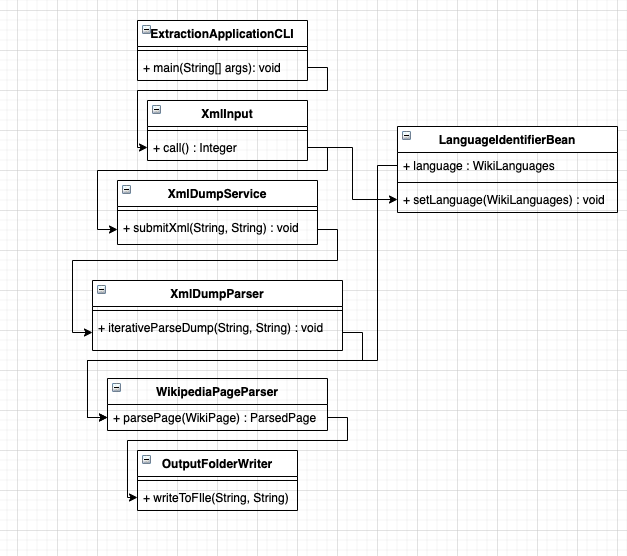
\includegraphics[width=1.0\linewidth]{framework_class_diagram}
	\caption{Framework Main Class Diagram}
	\label{fig:frameworkclassdiagram}
\end{figure}


\section{Implementation}

\subsection{Tools and libraries}

The chosen language for framework development is Java, as it is used in DBpedia Extraction Framework, described in section \ref{dbpedia_in_extraction_framework}. It is, however, important to notice that plain Java is not sufficient to achieve the goal of implementing modern Web Framework. For that reason, many other supplementary tools, libraries and other technologies were developed. This current ecosystem will be described below.

The project was developed using an IntelliJ IDEA\cite{intellij_link}, a modern  \gls{IDE} that is maintained by a Czech company JetBrains. The company is now also developing a JVM-based language called Kotlin, that will be able to overcome some of Java's own shortcomings, such as a lack of support for functional programming paradigm. For the current project, however, it was decided to eliminate unnecessary dependencies and use Java as a main development language. IntelliJ IDEA was used for development and testing of the framework.

\subsection{Spring Framework}

The Spring Framework is a Java platform that provides comprehensive infrastructure support for developing Java applications. Spring handles the infrastructure so you can focus on your application.Spring enables you to build applications from "plain old Java objects" (\gls{POJO}) and to apply enterprise services non-invasively. This capability applies to the Java Standard Edition programming model and to full and partial Java Enterprise Edition\cite{spring_ref}.

There is a several versions of Spring Framework, namely the original Spring and a newer version called Spring Boot. The difference between those two is that the original Spring leverages the use of \gls{XML} configurations, while Spring Boot instead uses Java Configuration classes. For the development, Spring Boot is used.

For this project, mostly prototype and singleton Bean scopes were used, with singleton being a default one.


\subsection{Java Jackson XML Library}\label{jackson_library}

The Jackson project is a collection of data processing tools for the Java language and the \gls{JVM} platform. It supports a wide range of data formats such as \gls{CSV}, Java Properties, XML, and \gls{YAML} through extension components that support the specific language.

The Jackson XML component is meant for reading and writing XML data by emulating how \gls{JAXB} works, although not conclusively.

In this project, Jackson library is used to serialize Java objects into XML and deserialize them back into Java objects, in order to eventually produce text output.

\paragraph{XmlMapper Class} 

XmlMapper is the main class from Jackson 2.x that helps the developers  in serialization. This mapper is available in jackson-dataformat-xml jar, that can be easily added to the project using Apache Maven - project's dependency management\cite{maven_project}.

An example of deserialization can be seen in Listing \ref{lst:xml-deserialization}. Here, a Mediawiki class is a \gls{POJO} class, or in other words a simple mapping of an XML scheme to a Java class hierarchy, where every subcomponent of a schema is mapped to a Java subclass.

\begin{lstlisting}[caption=Example of an XML Deserialization,frame=tlrb,  label = {lst:xml-deserialization}]{Name}
   
   private XmlMapper xmlMapper = new XmlMapper();
   
   private Mediawiki deserializeXml(String dump) throws IOException {
		return xmlMapper.readValue(dump, Mediawiki.class);
	}

\end{lstlisting}

\subsection{Article Parsing}\label{article_parsing}

The most important part of the Framework is a parsing component. While the code utilizes Jackson XML Library \ref{jackson_library} to deserialize XML, the article text is processed in a WikipediaPageParser class. First, we need to clean up the text from many tags used by Wikipedia\cite{Wikipedia_Template}.  Tags and patterns listed above utilize regular expressions to match and remove patterns in the text. The exact list of tags removed is described in the next list:

\begin{itemize}
	\item \textbf{Gallery.} Both tags(<gallery/>) and their contents are removed. 
	\item \textbf{Unit Conversion.}  For this tag, the Framework extracts 2nd and 3rd parts and separates them by a space, i.e. for "\{\{convert|2|km|mi\}\}" output is "2 km"
	\item \textbf{Emphasis.} Removes single-quote tags from text(''' or '') while keeping its contents intact.
	\item \textbf{No Table of Contents.} Remove technical "\_\_NOTOC\_\_" tags that hide table of contents.
	\item \textbf{Indentation.} Replaces excessive line breaks with simple \\n.
	\item \textbf{Math formula.} Remove all math formulas(<math>) and their contents.
	\item \textbf{IPA.} Removes all International Phonetic Alphabet(IPA) tags.
\end{itemize}

Regular expression is done using Java's Pattern class. In the example of a regular expression \ref{lst:code-regex} that is used  to remove gallery, the regular expression checks for a pattern <gallery>...</gallery>, ignoring cases and including line breaks as part of the .* regular expression, passing Pattern.DOTALL parameter.

\begin{lstlisting}[caption=Example of a regular expression,frame=tlrb,  label = {lst:code-regex}]{Name}
	private static final Pattern GALLERY = Pattern.compile("&lt;gallery&gt;.*?&lt;/gallery&gt;[\\n]?",
		Pattern.CASE_INSENSITIVE | Pattern.DOTALL);
\end{lstlisting}

\subsection{NIF Formatting}

After the article is parsed, the ParsedPage object is passed to the NifFormatter generator class methods to format output lines. This class utilizes Apache Jena modelling to create \gls{RDF} models, resources and properties. In the code listing \ref{lst:nif-format-context}, we can find the code that generates \gls{RDF} resources for DBPedia and context resourse, and then proceeds to create context's type property(http://persistence.uni-leipzig.org/nlp2rdf/ontologies/nif-core\#Context) and its starting index("0"\^\^<http://www.w3.org/2001/XMLSchema\#nonNegativeInteger>).

\begin{lstlisting}[caption=Generating Apache Jena context model,frame=tlrb,  label = {lst:nif-format-context}]{Name}
Resource dbPediaResource = jenaModel.createResource(dbpediaUrl);
Resource contextResource = jenaModel.createResource(PERSISTENCE_ONTOLOGY_LINK + "#" + LinkType.CONTEXT.getCapitalizedTypeLabel());

// Context NIF type
Property rdfSyntaxProperty = jenaModel.createProperty(RDF_SYNTAX_TYPE);
dbPediaResource.addProperty(rdfSyntaxProperty, contextResource);
// Context beginIndex
Property beginIndexProperty = jenaModel.createProperty(PERSISTENCE_ONTOLOGY_LINK, "#"+BEGIN_INDEX);
dbPediaResource.addProperty(beginIndexProperty, jenaModel.createTypedLiteral(beginIndex, XSDDatatype.XSDnonNegativeInteger));
\end{lstlisting}

NifFormatter converts parse page objects into Apache Jena models. For each article, three different models are produced: context model, page structure model and links model. Many of the strings required to generate the model are hardcoded, such as links(DBPedia URL, ontology) or property names. 

Context and Link model creation is straightforward, but page structure is more complicated. Page structure generation is done using a  recursive function. Main method is generatePageStructureEntry, and this method calls a recursive function generateNodeEntry for the article's root section. Then a recursive call processes every paragraph of the section, adding them as section resource properties with property name "hasParagraph". First and last paragraph have to be added as separate properties, so first and last paragraphs are added twice with "firstParagraph" and "lastParagraph" properties as well as again with "hasParagraph".  After processing all section's paragraph, every subsection of a section is then processed by recursive call. Subsections then are constructed with the same algorithm, until all the article's sections are processed.


\subsection{Output generation}

OutputFolderWriter is a simple class that utilizes java.io to produce output in the desired folder. The path to the folder is passed via --output CLI variable, and OutputFolderWriter creates three files in the folder: nif\_context.nt for article's context resources, nif\_links.nt for article's links and nif\_structure.nt for article's section structure. If the output folder is not created yet, the framework will create it. When the framework processes several articles, OutputFolderWriter iteratively appends output of every article to the files.

\subsection{Dynamic Language Support}\label{dynamic_lang_support}

The XML-structure of the Wikipedia article does not differ much from language to language. There are only a few points to be aware of: Footer headings and categories. In English, those would be "See also", "References", "Further reading", "External Links", and "Related pages", and Categories simply have a heading "Category". Those are the parts that have to be removed from the articles.

One of the project's requirements was to implement an easy extensibility mechanism to add new languages, mention in the Requirements Section \ref{framework_requirements}. This was achieved by adding an abstract class \lstinline{LanguageFooterRemover}. This class has some general functions to parse parts of the text that might be unique to different languages. Before the framework starts, it processes the configuration file language\_list.xml that is stored in the configuration folder. The examples of this file's contents can be seen in Listing \ref{lst:language-list}. Such template can easily be reused to extend the number of supported languages if needed.

\begin{lstlisting}[caption=Example of an language configuration file,frame=tlrb,  label = {lst:language-list}]{Name}
<languageContainer>
	<language>
		<langName>ENGLISH</langName>
		<categoryName>Category</categoryName>
		<footer>See also</footer>
		<footer>References</footer>
		<footer>Further reading</footer>
		<footer>External Links</footer>
		<footer>Related pages</footer>
	</language>
	<language>
	<langName>POLISH</langName>
		<categoryName>Kategoria</categoryName>
		<footer>Przypisy</footer>
		<footer>Uwagi</footer>
	</language>
</languageContainer>
\end{lstlisting}

\chapter{Testing and Results}

The main machine that was used for testing, unless specified otherwise, had next specifications:
\begin{itemize}
	\item \textbf{Processor:} 2,7 Hz Dual-Core Intel Core i5;
	\item \textbf{Memory:} 8 GB 1867 MHz DDR3;
	\item \textbf{Graphics Card:} Intel Iris Graphics 6100 1536 MB;
	\item \textbf{Operating System:} macOS Catalina, Version 10.15.6.
\end{itemize}

\paragraph{Project benchmarks}

\textbf{Benchmark Testing} measures a repeatable set of quantifiable results that serves as a point of reference against which products/services can be compared. The purpose of benchmark testing results is to compare the present and future software releases with their respective benchmarks.

A benchmark must be repeatable. For instance, with every iteration of load a test, if the response times varies too much, system performance be benchmarked. Response time needs to be stable amongst different load conditions.

A benchmark must be quantifiable. For example, the user experience cannot be quantified in numbers, but time a user spends on a webpage due to good UI can be quantified.

Next benchmark tests were repeatedly used to test the framework. They are located in the project's folder \\documents:

\begin{itemize}
	\item 1 Page test, English language. Expected to be completed quickly and successfully.
	\item 257 pages, English language. Execution time is expected to be less than a minute.
	\item 6738 pages, English language. Execution time is expected to be around 5 minutes.
	\item 6649 pages, Polish language. Execution time is expected to be around 5 minutes.
	\item 15118 pages, English language. Execution time is around 25 minutes.
\end{itemize}


Benchmarking can be used not only for performance testing, but also for testing the quality of output. While testing this project, the results were constantly compared to an ideal output, that has been provided by the DBpedia project\cite{dbpedia_url}. Dbpedia website contains ideal output format on  the resources page at https://www.dbpedia.org/resources/nif/. The output on the page is shown for the Antropology page in Turtle format, but it can be used to compare output properties for context, links and page structure.

Three different output components were compared separately. On the listings below, the ideal result can be seen, for the context output in Listing \ref{lst:context-example} - the output containing properties for the context. For links in Listing \ref{lst:links-example}, the example contains output for one of the phrases for "Austroasiatic languages" page. For page structure in Listing \ref{lst:page-structure-example}, the output shows an example of a Section and its reference to the parent context resource.

\begin{lstlisting}[caption=Exemplary result for NIF Context,frame=tlrb,  label = {lst:context-example}]{Name}
<http://dbpedia.org/resource/Anarchism?dbpv=2020-02&nif=context> <http://persistence.uni-leipzig.org/nlp2rdf/ontologies/nif-core#isString> "Anarchism is a radical political ... \n* Textbooks from Wikibooks  \n* Data from Wikidata  \n* Anarchy Archives. Anarchy Archives is an online research center on the history and theory of anarchism" .
\end{lstlisting}

\begin{lstlisting}[caption=Exemplary result for NIF Links,frame=tlrb,  label = {lst:links-example}]{Name}
<http://dbpedia.org/resource/Austroasiatic_languages?dbpv=2016-04&nif=phrase_94_109> <http://www.w3.org/1999/02/22-rdf-syntax-ns#type> <http://persistence.uni-leipzig.org/nlp2rdf/ontologies/nif-core#Phrase> .
<http://dbpedia.org/resource/Austroasiatic_languages?dbpv=2016-04&nif=phrase_94_109> <http://persistence.uni-leipzig.org/nlp2rdf/ontologies/nif-core#referenceContext> <http://dbpedia.org/resource/Austroasiatic_languages?dbpv=2016-04&nif=context> .
<http://dbpedia.org/resource/Austroasiatic_languages?dbpv=2016-04&nif=phrase_94_109> <http://persistence.uni-leipzig.org/nlp2rdf/ontologies/nif-core#beginIndex> "94"^^<http://www.w3.org/2001/XMLSchema#nonNegativeInteger> .
<http://dbpedia.org/resource/Austroasiatic_languages?dbpv=2016-04&nif=phrase_94_109> <http://persistence.uni-leipzig.org/nlp2rdf/ontologies/nif-core#endIndex> "109"^^<http://www.w3.org/2001/XMLSchema#nonNegativeInteger> .
<http://dbpedia.org/resource/Austroasiatic_languages?dbpv=2016-04&nif=phrase_94_109> <http://persistence.uni-leipzig.org/nlp2rdf/ontologies/nif-core#superString>
\end{lstlisting}

\begin{lstlisting}[caption=Exemplary result for NIF Page Structure,frame=tlrb,  label = {lst:page-structure-example}]{Name}
<http://dbpedia.org/resource/Ada?dbpv=2016-04&nif=section_0_17> <http://www.w3.org/1999/02/22-rdf-syntax-ns#type> <http://persistence.uni-leipzig.org/nlp2rdf/ontologies/nif-core#Section> .
<http://dbpedia.org/resource/Ada?dbpv=2016-04&nif=section_0_17> <http://persistence.uni-leipzig.org/nlp2rdf/ontologies/nif-core#beginIndex> "0"^^<http://www.w3.org/2001/XMLSchema#nonNegativeInteger> .
<http://dbpedia.org/resource/Ada?dbpv=2016-04&nif=section_0_17> <http://persistence.uni-leipzig.org/nlp2rdf/ontologies/nif-core#endIndex> "17"^^<http://www.w3.org/2001/XMLSchema#nonNegativeInteger> .
<http://dbpedia.org/resource/Ada?dbpv=2016-04&nif=section_0_17> <http://persistence.uni-leipzig.org/nlp2rdf/ontologies/nif-core#referenceContext> <http://dbpedia.org/resource/Ada?dbpv=2016-04&nif=context> .
...
\end{lstlisting}

The output format should be in N-triples\cite{ntriples_format}, better described in Section \ref{rdf-description}.

\section{Smoke Testing}

Smoke test  is a test or a test suite that covers the main functionality of a component or system to determine whether it works properly before planned testing begins\cite{smoke_testing}.

To list the information, those are the advantages of an early and continuous smoke testing:
\begin{itemize}
	\item It exposes any integration issues, that is if there any problems in communication between different tools used in the project.
	\item It uncovers problems early, 
	\item It provides some level of confidence that changes to the software have not adversely affected major areas (the areas covered by smoke testing)
\end{itemize}

This kind of testing was performed during every stage of the implementation after each new part of functionality has been added to the framework. It includes \gls{CLI} testing, API testing, functionality testing, and output verification. During development and testing the framework was running locally on a Mac-based machine.

A big amount of bugs and errors was revealed and subsequently fixed during these tests. For example, there were many errors related to the parsing of Wikipedia articles, and lots of inconsistencies happening during the page structure translation into the page. 

Furthermore, scaling the framework has caused a lot of problems. The size of an English Wikipedia dump is about 16 GB of data, and parsing it takes a lot of time. During those tests, it was discovered that such amount of data can not be handled by the server, and therefore an adequate API for production purposes can not be easily provided.

For the smoke testing, the next tests were conducted:

\begin{itemize}
	\item Single-article XML dump in English language.
	\item Two-page XML dump in English language.
	\item Other languages support testing, conducted for a single page from a German segment of Wikipedia.
\end{itemize}




\section{Unit Test coverage}

Unit testing is a software testing method by which individual units of source code - sets of one or more computer program modules together with associated control data, usage procedures, and operating procedures - are tested to determine whether they are fit for use. The goal of unit testing is to isolate each part of the program and show that the individual parts are correct. A unit test provides a strict, written contract that the piece of code must satisfy. As a result, it affords several benefits\cite{kh07}.

Unit testing finds problems early in the development cycle. This includes both bugs in the programmer's implementation and flaws or missing parts of the specification for the unit. The process of writing a thorough set of tests forces the author to think through inputs, outputs, and error conditions, and thus more crisply define the unit's desired behavior. The cost of finding a bug before coding begins or when the code is first written is considerably lower than the cost of detecting, identifying, and correcting the bug later. Bugs in released code may also cause costly problems for the end-users of the software. Code can be impossible or difficult to unit test if poorly written, thus unit testing can force developers to structure functions and objects in better ways\cite{bp88}\cite{test_early}\cite{prove_it_works}.

An important indicator for the quality of tests is their code coverage. Code coverage is measured by what percentage of the code is tested by unit tests. Running an analysis shows that  73\% of the current Framework lines, 53\% of its methods, or 52\% of its classes are covered by tests. Both unit and integration tests are included into this statistic, as the analysis tool does not differentiate those tests.


\subsection{JUnit Framework}

For the framework implementation, a JUnit library was used. \textbf{JUnit} is a  popular Testing Framework used to implement unit tests in Java\cite{junit_framework}.

For a given project, unit tests were used to test the execution of a WIkipediaPageParser class, that is used to parse separate pages, as well as its supplementary classes, such as a DumpSplitService. You can see the examples of a unit test used in the project in the Listing\ \ref{lst:unit-test-example}:


\begin{lstlisting}[caption=JUnit Paragraph Parsing Unit Test Class,frame=tlrb,  label = {lst:unit-test-example}]{Name}
@Log4j
public class WikipediaPageParserTest {

	private static WikipediaPageParser pageParser;
	private static WikiPage wikiPage;
	private static XmlTransformer contextLanguageTransformer;
	
	@BeforeAll
	public static void beforeAll() throws IOException {
		pageParser = new WikipediaPageParser(new ContextLanguageTransformer());
		
		URL textUrl = Resources.getResource("page_test.txt");
		wikiPage = new WikiPage("Anarchism",
		Resources.toString(textUrl, StandardCharsets.UTF_8));
	}
	
	@Test
	public void parseParagraphsTest() throws IOException, ParsingException {
		Subdivision root = pageParser.buildPageStructure(wikiPage);
		// check that the paragraphs are parsed
		assertTrue(root.getParagraphs().size() > 1);
		// check that the page has a meaningful structure
		assertTrue(root.getChildren().size() > 1);
	}
	...
}
\end{lstlisting}

Those tests are checking for specific methods to return some basically expected values, as well as test possible corner cases that were previously discovered as bugs, but were already fixed later. Such tests can be classified as regression tests.  For example, Listing \ref{lst:regression-test-example} is a test that checks whether <ref> tags are removed from the text by the WikiTagsRemover class. Those tags were initially causing issues with parsing, and a unit test has been added to check whether they are properly removed. If the WikiTagsRemover method is broken during development, the test will immediately indicate that method's output is now broken(or that a "regression" has happened). Those tests are run on every project recompilation.

\begin{lstlisting}[caption=Regression Testing,frame=tlrb,  label = {lst:regression-test-example}]{Name}
@Test
public void removeRefTags() {
	String refText = "&lt;ref&gt;{{cite OED|anarchism}}&lt;/ref&gt; and the <ref>word</ref> &lt;ref&gt;{{cite OED|anarchism}}&lt;/ref&gt;";
	refText = StringEscapeUtils.unescapeHtml4(StringEscapeUtils.unescapeHtml4(refText));

	Pattern HTML_TAGS = Pattern.compile("<[^>]+>");
	refText = wikiTagsRemover.removeHtmlTags(refText);
	log.info(refText);
	Assert.assertFalse(HTML_TAGS.matcher(refText).find());
}
\end{lstlisting}

\section{Integration Testing}

Integration testing is used to test application as a whole, running through separate modules in one test \cite{integration_test1}. In contrast to the unit tests that only focus on an individual module, integration tests make sure that the application can accept input, process it, and then produce output\cite{integration_test2}. This output is then verified against the test data for correctness.


Integration testing in the project tests that all aspects of the Framework work as intended, from parsing to output, and different cases with varying sizes and languages are automatically tested whenever the project is recompiled. To speed up the development, it is possible to skip those tests by compiling the project with -DskipTests argument, but this is not recommended. Integration tests compare Framework's output for prepared articles that are stored in the test folder with expected values that are manually verified to be true. 

Integration tests are placed in the OutputValidationTests class. Every test is verifying any specific information:

\begin{itemize}
	\item \textbf{test*ArticleGeneral} - tests that the total amount of nodes/lines in the context, structure and links files is correct;
	\item \textbf{test*ArticleContext} - tests context output file to verify that every node and property is in the output;
	\item \textbf{test*ArticleLinks} - tests if the links output file is formed correctly. Since there is a lot of links in every article, only selected links are tested;
	\item \textbf{test*ArticleStructure} - tests if the page structure output file is formed correctly. Similarly to links, this test verifies that a selected part of sections are correctly formed in the output.
\end{itemize}

Apache Jena is used to parse the output and create a model. The model is then verified by the integration test, as can be seen on Listing \ref{lst:integration-test-example}:

\begin{lstlisting}[caption=Integration Testing - English Article Context,frame=tlrb,  label = {lst:integration-test-example}]{Name}
    @Test
public void testEnglishArticleContext() throws IOException {
	loadArticle("xml_test_page.xml", "ENGLISH");
	
	File outputContext = Paths.get(folder.getRoot().getAbsolutePath(), OutputFolderWriter.CONTEXT_FILENAME).toFile();
	
	jenaModel.read(new FileInputStream(outputContext), null, NTRIPLES);
	
	String testSubject = String.format("http://dbpedia.org/resource/Anarchism?dbpv=%s&nif=context"
	, getCurrentDateString());
	String testPredicate = "http://www.w3.org/1999/02/22-rdf-syntax-ns#type";
	String testObject = getPersistenceOntologyUrl("Context");
	
	// test if type is Context
	assertStatementContains(testSubject, testPredicate, testObject);
		
	....
	
	// test predLang
	assertStatementContains(testSubject, testPredicate, testObjectLiteral);
	
	testPredicate = getPersistenceOntologyUrl("sourceUrl");
	testObjectLiteral = createLiteral("http://en.wikipedia.org/wiki/Anarchism");
	
	//test sourceUrl
	assertStatementContains(testSubject, testPredicate, testObjectLiteral);
	
	jenaModel.removeAll();
}
\end{lstlisting}

Integration tests also verify that other languages are properly processed. Currently integration tests cover English and German languages. For a German article, integration test on Listing \ref{lst:integration-test-german} verifies that language input parameter is processed correctly and the context output specifies the correct language:

\begin{lstlisting}[caption=Integration Testing - German Article Context,frame=tlrb,  label = {lst:integration-test-german}]{Name}
    @Test
public void testGermanArticleContext() throws IOException{
	loadArticle("xml_test_deutsch_one_page.xml", "GERMAN");
	....
	
	testPredicate = getPersistenceOntologyUrl("predLang");
	Literal testObjectLiteral = createLiteral("http://lexvo.org/id/iso639-3/deu");
	
	// test predLang
	assertStatementContains(testSubject, testPredicate, testObjectLiteral);
}
\end{lstlisting}


\section{End-to-End Testing}\label{end_to_end_testing}

\textbf{End-to-end testing} is a Software testing methodology to test an application flow from start to end. The purpose of End-to-end testing is to simulate the real user scenario and validate the system under test and its components for integration and data integrity. What it means for this project is that we will need to do a test from downloading an XML dump from Wikipedia to receiving the processed results. Here is the general outlay of a testing process:

\begin{enumerate}
	\item Download the latest Wikipedia dump\cite{wikimedia_downloads}. They are released at least monthly and usually twice a month. Different languages are listed after the metawiki dumps.
	\item Unzip the file, in Unix-like operating systems usually done in \lstinline{bzip2 -d wikidatawiki-*-pages-meta-history1.xml-p1p224.bz2} 
	\item [Optional] Because parsing of the whole XML dump is time-consuming, I have used a way to reduce the amount of articles that is processed. To do it, it is possible to execute this command \lstinline{head -n 100000 enwiki-20191101-pages-articles-multistream1.xml > short_test_100k.xml}, and then properly close off the XML by removing the last article and close the XML brackets.
	\item Build the framework and pass the input parameters to a file. I have created a script \lstinline{parse_xml_dump.sh} that will build the framework if necessary and run the executable with the XML dump path as the parameter.
\end{enumerate}


\subsection{SHACL Shape Validation}

To ensure that \gls{RDF} resources produced are not malformed, \gls{SHACL} forms were utilized. \gls{SHACL} shapes allow to define certain classes for \gls{RDF} resources and then to validate any \gls{RDF} resources against those shapes, making it possible to run the tests on any output.
In the Listing \ref{lst:shacl-class} a definition for a Context class is shown. \gls{SHACL} definitions are defined in a Turtle format, which is another format from  \gls{NIF} format, produced by the framework.
\begin{lstlisting}[caption=SHACL Context Class definition,frame=tlrb,  label = {lst:shacl-class}]{Name}]
ontology:Context
rdf:type rdfs:Class ;
rdfs:label "Context" ;
.

ontology:isString
rdf:type rdf:Property ;
rdfs:domain ontology:Context ;
rdfs:label "Context string" ;
rdfs:range xsd:string ;
.
...
ontology:ContextShape
a sh:NodeShape ;
sh:targetClass ontology:Context ;
sh:property ontology:isStringShape ;
sh:property ontology:sourceUrlShape ;
sh:property ontology:predLangShape ;
sh:property ontology:beginIndexShape ;
sh:property ontology:endIndexShape ;
.

ontology:isStringShape
a sh:isStringShape ;
sh:path ontology:isString ;
sh:minCount 1 ;
sh:maxCount 1 ;
sh:datatype xsd:string ;
sh:severity sh:Violation
.
\end{lstlisting}

To validate output against SHACL shapes, various tools can be used, notably an open-source validator to test shapes and data: https://shacl.org/playground/. Application's output can be converted to a Turtle format using EasyRDF Converter from https://www.easyrdf.org/converter/.

Current SHACL shapes validate whether properties are present and that their number does not exceed the required number. For more complex validation, integration tests are used.

\subsection{English language parsing}

Initially the testing was done on a single English-language article. This testing uncovered many problems with the parsing model, such as the need to update the recursive function to build the page structure. Most importantly, the first testing helped to understand the vast number of Wikipedia XML components. Of those, I had to drop the parts that were already covered by the previous frameworks mentioned in Section \ref{dbpedia_in_extraction_framework}, such as infoboxes, images, files, categories and others, and instead focus only on the text. I also dropped the citations mentioned in the article's footer, and instead focused on the text itself.

In the Listing \ref{lst:english-cli}, an example of the Framework's output is shown. Every run shows the total amount of pages parsed, as well as what percentage of articles was not parsed due to Framework's exceptions. In this case 96.74\% of articles were parsed and added to the output. If there is a processing error, it is indicated in the output by providing the reason for an error and part of the paragraph where the error happened, for example "Error parsing page Crankshaft: Broken xml component - closing brace not found for \{\{ in paragraph \{\{Main|Science and t...".

\begin{lstlisting}[caption=Example of an English processing command,frame=tlrb,  label = {lst:english-cli}]{Name}]
macs-MacBook-Air:wiki-realtime-extractor mac$    ./parse_xml_dump.sh documents/large_documents/short_test_1000k.xml --language=ENGLISH --clean -o=output
....
22-01-31 00:08:36 INFO  XmlDumpParser:112 - Parsed page: Cemetery H culture
2022-01-31 00:08:36 INFO  XmlDumpParser:112 - Parsed page: Corrado Gini
2022-01-31 00:08:36 ERROR XmlDumpParser:121 - Error parsing page Crankshaft: Broken xml component - closing brace not found for "{{" in paragraph "{{Main|Science and t..."
2022-01-31 00:08:36 INFO  XmlDumpParser:112 - Parsed page: Central nervous system
2022-01-31 00:08:36 INFO  XmlDumpParser:112 - Parsed page: Caste
2022-01-31 00:08:36 INFO  XmlDumpParser:112 - Parsed page: Creation
2022-01-31 00:08:36 INFO  XmlDumpParser:112 - Parsed page: Coral 66
2022-01-31 00:08:36 INFO  XmlDumpParser:112 - Parsed page: Rhyming slang
2022-01-31 00:08:36 INFO  XmlDumpParser:112 - Parsed page: Canchim
2022-01-31 00:08:36 INFO  XmlDumpParser:135 - Total pages parsed: 3378. Success rate: 96.74%. Seconds passed: 198
\end{lstlisting}

\subsection{Testing other languages}

Additionally to English language, I have added other popular Wikipedia languages. According to the latest Wikipedia statistics, those are the main languages of Wikipedia\cite{top_ten_wikis}:

\begin{enumerate}
	\item \textbf{English:} 2,567,509 articles, 22.5\% of the total number of articles;
	\item \textbf{German:} 808,044 articles, 7.1\%;
	\item \textbf{French:} 709,312 articles, 6.2\%;
	\item \textbf{Polish:} 539,688 articles, 4.7\%;
	\item \textbf{Japanese:} 523,629 articles, 4.6\%.
\end{enumerate}

Dynamic Language Support is described in \ref{dynamic_lang_support}. To verify that the Framework works in other languages, I have downloaded English, German and Polish XML dumps and run the framework against them, as seen on Listing \ref{lst:polish-cli}. 


\begin{lstlisting}[caption=Example of a Polish processing command,frame=tlrb,  label = {lst:polish-cli}]{Name}]
macs-MacBook-Air:wiki-realtime-extractor mac$    ./parse_xml_dump.sh documents/xml_test_polish.xml --language=POLISH --clean -o=output
2022-01-31 00:00:35 INFO  XmlDumpParser:112 - Parsed page: AWK
2022-01-31 00:00:36 INFO  XmlDumpParser:112 - Parsed page: Alergologia
2022-01-31 00:00:37 INFO  XmlDumpParser:112 - Parsed page: Aksjomat
2022-01-31 00:00:37 INFO  XmlDumpParser:112 - Parsed page: Arytmetyka
....
2022-01-31 00:00:40 INFO  XmlDumpParser:112 - Parsed page: Alabama
2022-01-31 00:00:40 INFO  XmlDumpParser:135 - Total pages parsed: 76. Success rate: 100.00%. Seconds passed: 5
\end{lstlisting}


\subsection{Output format validation}

There are several utilities that can be used to validate the output, most notable Apache Jena and rapper\cite{rapper_utility}. For the output validation, I have picked rapper, as it is more lightweight and has the ability to count or parse the provided N-triples. For example, the command \lstinline{rapper --input ntriples --output rdfxml --show-graphs nif\_links.nt} will parse the links and transform it into RDF/XML format. If this transformation will not throw any exceptions, this will mean that the output is a valid set of N-triples. Rapper tool can also be used to convert output into a different format, such as RDF.

\subsection{Scale Testing}

For the scale testing, I have implemented logging and a simple parsing success metric, as some of the articles have a syntax that may deviate from the standard or the framework's programmed expectations. For example, some might contain links that are broken with line separators, or differently encoded XML components. 

To further measure the time that the application will take to parse the code, I have added the execution time metric. To make sure it is still possible to execute, I added a --dry-run CLI option that cleans up the output files to remove output after every execution. Not doing that results in generating text that takes a lot of disk space. Unfortunately, output clean up slows down execution by around 3 times, so this option is unusuable for a general performance testing.

I have run several tests over the English Wiki dump with the next results. The table shows results with appending and keeping text in output files, that is faster because the file output connection is not closed after every article parsing.

\begin{tabular}{|c|c|c|c|}
	\hline
	\# of pages parsed & Total execution time &  ms per article &  Success rate\\
	\hline
	257 & 26 & 110 & 100\% \\
	\hline
	257 & 46 & 178 & 100\% \\
	\hline
	2087 & 109  & 50 & 88.5\% \\
	\hline
	6738 & 237  & 35 & 87.9\% \\
	\hline
	6649 & 414  & 63 & 96.35\% \\
	\hline
	15118 &  1433 & 94 & 96.47\% \\
	\hline
\end{tabular}

\chapter{Conclusions}

The result of this thesis is a Java Framework that allows users to parse and retrieve the Wikipedia XML dump and achieves most of the original objectives, in some places with a room for improvement:
\begin{enumerate}
	\item \textbf{Accept and process input data in the form of Wikipedia XML dumps.} The Wikipedia XML Dump parsing was achieved, and the process to do so best described in Section \ref{end_to_end_testing}. The statistics show that the parsing success rate averages on 88\% over the large amounts of articles, meaning that around 12\% of articles will contain some kind of component that will not be parsable by the framework and will be skipped. These systemic errors can be avoided by further investigation of Wikipedia's XML Format.
	\item \textbf{Extract context.} Context is extracted and stored in the form of N-Triples. Some of the contexts might still contain traces of the original XML code. This can be later fixed by improving the XML removal code.
	\item \textbf{Extract page structure.} Page structure is extracted and recursively built in the form of N-Triples.
	\item \textbf{Extract links.} Links are extracted, URLs that link them to the page structure are created.
	\item \textbf{Provide outputs for context, links and page structure in the form of N-Triples.} Output is printed.
	\item \textbf{Implement language extensibility.} Language extensibility mechanism is implemented, new languages can be added in the form of an XML that is parsed into \gls{POJO} when the application is starting, better described in Section \ref{dynamic_lang_support}. Framework is tested in several languages - English, German and Polish.
	\item \textbf{Provide a user interface.} User interface is provided in two different forms and is described in Section \ref{usability_considerations}.
\end{enumerate} 


\section{Future improvements}

There is a number of future improvements that can be done to this project:

\begin{itemize}
	\item Code quality improvements. There is currently some unused code, style warnings and duplicate fragments that can be updated to clean up the code.
	\item Article parsing success rate. By analyzing the logs, more articles can be successfuly parsed by adding more rules to regular expression editing of the context.
	\item Add parsing of Wikipedia footers. Only the main article text is currently parsed by the Framework, the footers, specifically citations, might contain useful information.
	\item Add horizontal scalability. Execution on the main Wikipedia dump files takes a lot of time, with 25 minutes for each XML part and 27 parts available for English, the whole processing can take around 10 to 11 hours. The work, however, can be easily parallelized by splitting the input to be processed by different machines.
\end{itemize}

\printglossaries

\bibliographystyle{iso690.bst}
\bibliography{ref}


\end{document}
